\section{The MSL Radiation Assessment Detector}
\label{sec:mslrad}

Built in a cooperation between the University of Kiel and Southwest Research Institute, the \acl{RAD}\acused{RAD} \citep[\acs{RAD},][]{Hassler-2012-MSLRAD} instrument onboard the \acl{MSL}\acused{MSL} \citep[\acs{MSL},][]{Grotzinger-2012} mission provided the first-ever direct radiation measurements on the surface of Mars. It is designed to measure both charged and neutral particles, and calculate particle spectra as well as dosimetric quantities, such as the \ac{TID} rate and \ac{LET} spectra. This aligns with its main science objectives, which include the characterization of energetic particle spectra on the surface of Mars (\acp{GCR} and \acp{SEP}) and the determination of the radiation hazard for past and present life on Mars and for future human Mars missions. Consequently, \ac{RAD} not only been continuously measuring the radiation environment on the Martian surface since the \textit{Curiosity} rover's landing on August 6, 2012, but has also been active during a large part of the 9-month flight to Mars (the so-called cruise phase) to evaluate the radiation dose that astronauts would receive on a flight to Mars.

\begin{figure}
	\centering
	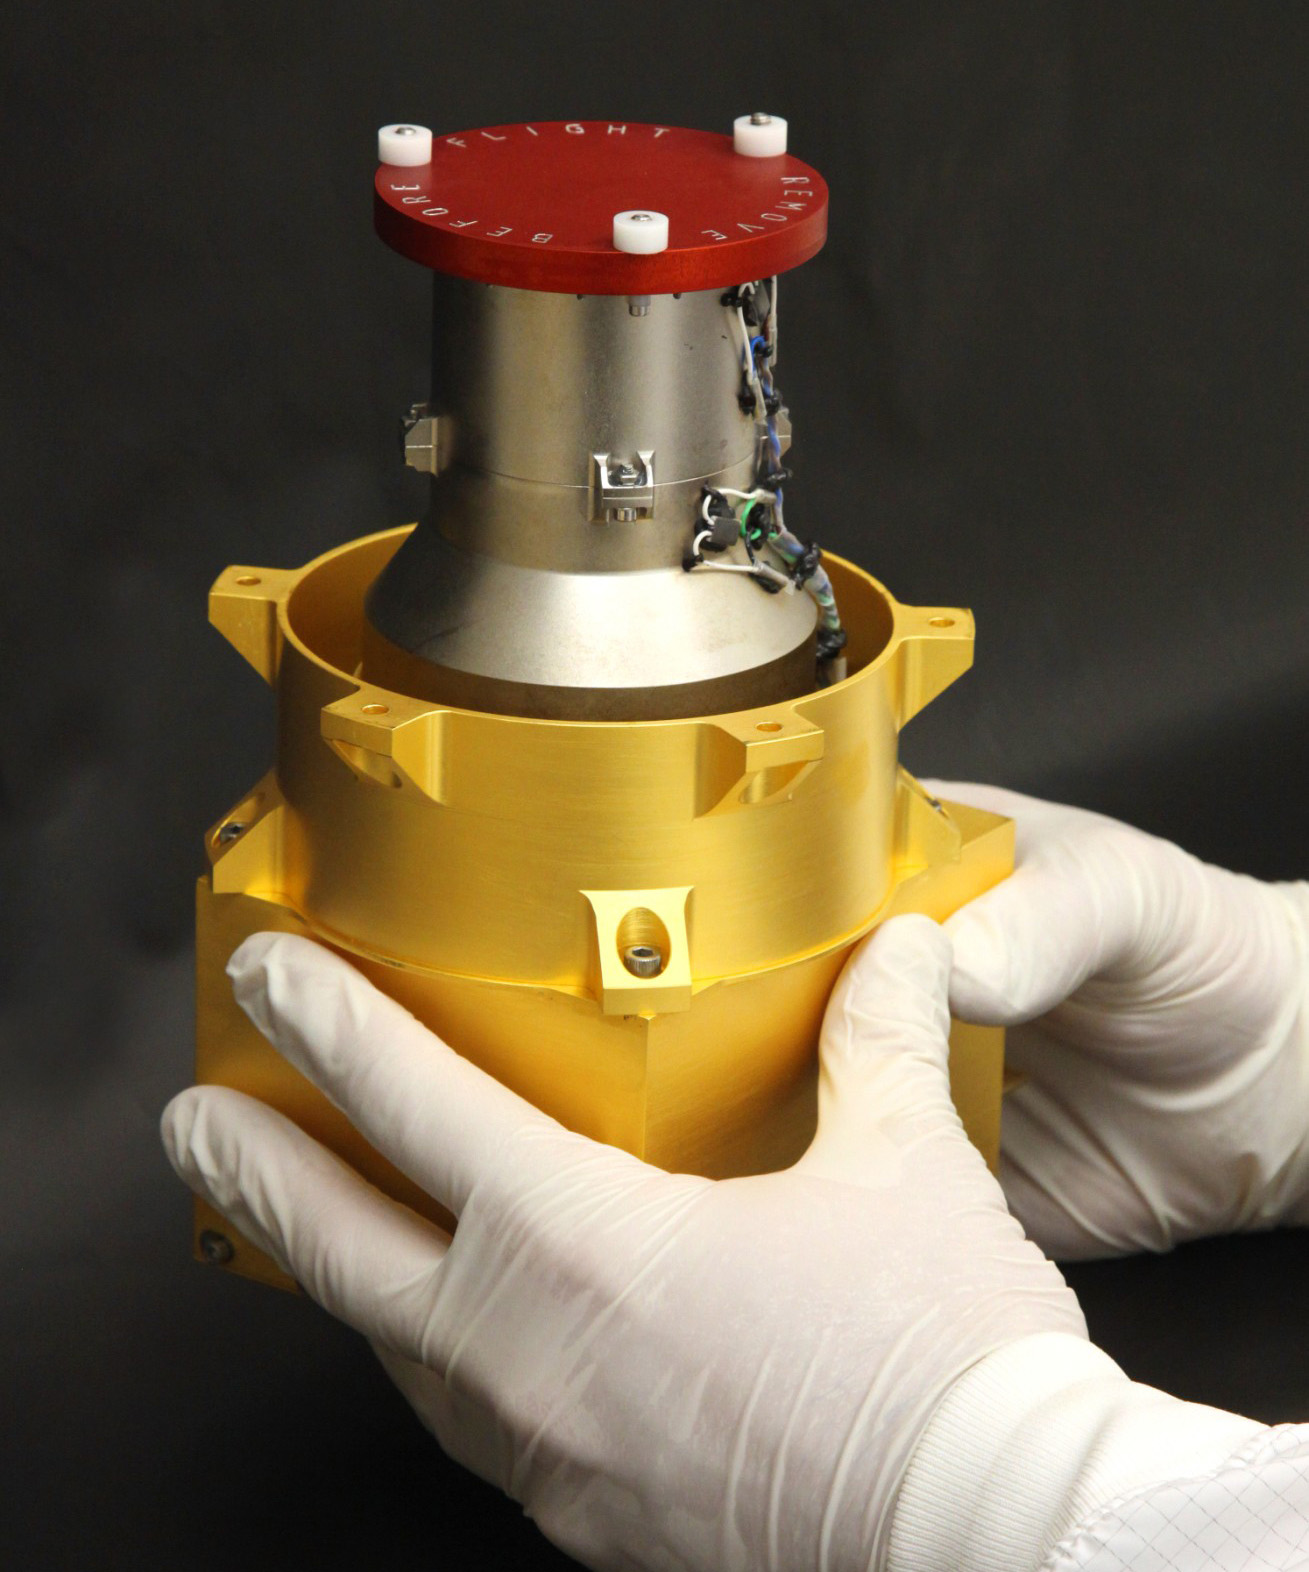
\includegraphics[width=0.4\linewidth]{images/rad}
	\caption[Photo of the \acs{RAD} sensor head]{A photo of the \ac{RAD} sensor head before it was mounted on the \ac{MSL} spacecraft. Source: NASA/JPL-Caltech/SwRI}
	\label{fig:rad-photo}
\end{figure}

The \ac{RAD} sensor head (shown in \autoref{fig:rad-photo}) is mounted on the top deck of the rover, pointing towards the zenith. It is composed of three hexagonal silicon solid-state detectors (A, B, and C) with a thickness of \SI{300}{\micro\meter}, mounted on top of each other to form a charged particle telescope (\autoref{fig:rad-sensorhead}) with an opening angle of about \SI{60}{\degree}. Each detector is split into inner and outer segments.
Directly below the charged particle telescope follows the D detector, a cesium iodide (CsI) scintillator in the shape of a truncated hexagonal pyramid. Its shape is chosen so that it continues the opening angle of the charged particle telescope (shown with dashed lines in \autoref{fig:rad-sensorhead}). The E detector, which is located below D, is a plastic scintillator and mainly responsible for neutral particle detection. D and E are surrounded by another plastic scintillator (F), which is used as an anticoincidence shield to reject ions that enter D or E from the sides.

\begin{figure}
	\centering
	%\documentclass{standalone}
%\usepackage{tikz}
%\usepackage{amsmath}

%\usetikzlibrary{calc}
%\usetikzlibrary{decorations.pathmorphing}

%\definecolor{light-gray}{gray}{0.9}

%\begin{document}
\begin{tikzpicture}[scale=0.8]
    \tikzset{%
        add/.style args={#1 and #2}{
            to path={%
                ($(\tikztostart)!-#1!(\tikztotarget)$)--($(\tikztotarget)!-#2!(\tikztostart)$)%
                \tikztonodes},add/.default={.2 and .2}}
    }  
    
    \def\bottomwidth{3.25}
    \def\midwidth{1.8}
    \def\topwidth{1.65}
    \def\bottomheight{2.5}
    \def\midheight{4.375}
    \def\Fthickness{1}
    \def\Sithickness{0.1}
    \def\BCdistance{0.15}
    \def\topheight{8.375}
    
    % FOV
    \draw[add=0 and 0.3, dashed] (\midwidth - \Fthickness, \midheight) to (-\topwidth, \topheight);
    \draw[add=0 and 0.3, dashed] (-\midwidth + \Fthickness, \midheight) to (\topwidth, \topheight);

    % A
    \draw[fill=light-gray] (-\topwidth, \topheight - \Sithickness) rectangle (\topwidth, \topheight);
    \draw (-\midwidth + \Fthickness, \topheight - \Sithickness) --  (-\midwidth + \Fthickness, \topheight);
    \draw (-\midwidth + \Fthickness, \topheight - \Sithickness) --  (-\midwidth + \Fthickness, \topheight);
    \draw (\midwidth - \Fthickness, \topheight - \Sithickness) --  (\midwidth - \Fthickness, \topheight);
    \draw (\midwidth - \Fthickness, \topheight - \Sithickness) --  (\midwidth - \Fthickness, \topheight);
    \draw[latex-] (-\topwidth, \topheight - \Sithickness / 2) -- (-\topwidth - 0.5, \topheight - \Sithickness / 2) node[left] {A};
    
    % B
    \draw[fill=light-gray] (-\topwidth, \midheight + \BCdistance) rectangle (\topwidth, \midheight + \BCdistance + \Sithickness);
    \draw (-\midwidth + \Fthickness, \midheight + \BCdistance) --  (-\midwidth + \Fthickness, \midheight + \BCdistance + \Sithickness);
    \draw (-\midwidth + \Fthickness, \midheight + \BCdistance) --  (-\midwidth + \Fthickness, \midheight + \BCdistance + \Sithickness);
    \draw (\midwidth - \Fthickness, \midheight + \BCdistance) --  (\midwidth - \Fthickness, \midheight + \BCdistance + \Sithickness);
    \draw (\midwidth - \Fthickness, \midheight + \BCdistance) --  (\midwidth - \Fthickness, \midheight + \BCdistance + \Sithickness);
    \draw[latex-] (-\topwidth, \midheight + \BCdistance + \Sithickness / 2) -- (-\topwidth - 0.5, \midheight + \BCdistance + \Sithickness / 2 + 0.3) node[left] {B};
    
    % C
    \draw[fill=light-gray] (-\topwidth, \midheight) rectangle (\topwidth, \midheight + \Sithickness);
    \draw (-\midwidth + \Fthickness, \midheight) --  (-\midwidth + \Fthickness, \midheight + \Sithickness);
    \draw (-\midwidth + \Fthickness, \midheight) --  (-\midwidth + \Fthickness, \midheight + \Sithickness);
    \draw (\midwidth - \Fthickness, \midheight) --  (\midwidth - \Fthickness, \midheight + \Sithickness);
    \draw (\midwidth - \Fthickness, \midheight) --  (\midwidth - \Fthickness, \midheight + \Sithickness);
    \draw[latex-] (-\topwidth, \midheight + \Sithickness / 2) -- (-\topwidth - 0.5, \midheight + \Sithickness / 2) node[left] {C};
    
    % border of ABC
    \draw (-\topwidth, \midheight) -- (-\topwidth, \topheight);
    \draw (\topwidth, \midheight) -- (\topwidth, \topheight);
    
    % D
    \draw[fill=light-gray] (\bottomwidth - \Fthickness, \bottomheight) --  (-\bottomwidth + \Fthickness, \bottomheight) -- (-\midwidth + \Fthickness, \midheight) -- (\midwidth - \Fthickness, \midheight) -- (\bottomwidth - \Fthickness, \bottomheight);   
    \node at (0, {\bottomheight + (\midheight - \bottomheight) / 2}) {D};   
    
    % E
    \draw[fill=green!50] (\bottomwidth - \Fthickness, \bottomheight) -- (\bottomwidth - \Fthickness, \Fthickness) --
    (-\bottomwidth + \Fthickness, \Fthickness) --  (-\bottomwidth + \Fthickness, \bottomheight) -- (\bottomwidth - \Fthickness, \bottomheight);  
    \node at (0, {\Fthickness + (\bottomheight - \Fthickness) * 0.4}) {E};   
    
    % F
    \draw[fill=yellow] (-\bottomwidth, 0) -- (\bottomwidth, 0) -- (\bottomwidth, \bottomheight) -- (\midwidth, \midheight) --
    (\midwidth - \Fthickness, \midheight) -- (\bottomwidth - \Fthickness, \bottomheight) -- (\bottomwidth - \Fthickness, \Fthickness) --
    (-\bottomwidth + \Fthickness, \Fthickness) --  (-\bottomwidth + \Fthickness, \bottomheight) -- (-\midwidth + \Fthickness, \midheight) --
    (-\midwidth, \midheight) -- (-\bottomwidth, \bottomheight) -- (-\bottomwidth, 0);     
    \node at (0, \Fthickness / 2) {F};
    
    % trajectories of ions
    \draw[thick, green, -latex] (-\topwidth*0.7, \topheight*1.15) node[above, align=center] {\small Ion\\ \small (accepted)}
     -- ({-(\midwidth - \Fthickness) * 0.5}, \midheight + \Sithickness / 2);
    \draw[thick, green, -latex] (\topwidth*0.65, \topheight*1.15) node[above, align=center] {\small Ion\\ \small (accepted)}
     -- ({-(\midwidth - \Fthickness) * 0.5}, {\bottomheight +  (\midheight - \bottomheight) / 2});
    \draw[thick, red, -latex] (0, \topheight*1.3) node[above, align=center] {\small Ion\\ \small (rejected)}
     -- (0, \topheight - \Sithickness / 2);
    \draw[thick, red, -latex] (\bottomwidth, \midheight) node[above right, align=center] {\small Ion\\ \small (rejected)}
    -- (\bottomwidth * 0.4, {\bottomheight + (\midheight - \bottomheight) * 0.2});
    
    % trajectory of neutron
    \draw[thick, gray, -latex] (-\bottomwidth*0.3, -0.5) node[below] {\small Neutron (accepted)}
    -- (-\bottomwidth*0.3, {\Fthickness + \bottomheight * 0.2});
    \draw[thick, gray, -latex]  (-\bottomwidth*0.3, {\Fthickness + \bottomheight * 0.2}) -- (-\bottomwidth * 1.1, \bottomheight * 1.3);
    \draw[thick, blue, -latex]  (-\bottomwidth*0.3, {\Fthickness + \bottomheight * 0.2}) -- (0, \bottomheight * 1.1) node[midway, right, xshift=1mm] {\small Recoil proton};
    
    % trajectory of gamma
    \draw[thick, gray, decorate, decoration=snake] (-\bottomwidth*1.2, \bottomheight * 0.8) node[below, align=center, xshift=-4mm] {\small $\gamma$-ray\\ \small (accepted)} -- (-\bottomwidth * 0.3, \bottomheight * 1.4);
    \draw[thick, gray, -latex] (-\bottomwidth * 0.3, \bottomheight * 1.4) -- ++ (\bottomwidth * 0.03, \bottomheight * 0.02);
    
\end{tikzpicture}
%\end{document}
	\caption[Schematic diagram of the \acs{RAD} sensor head]{Schematic diagram of the \ac{RAD} sensor head. Red, green and gray arrows show possible trajectories of charged and neutral particles through the detectors. Based on      \textcite{Hassler-2012-MSLRAD}, Fig. 7b}
	\label{fig:rad-sensorhead}
\end{figure}

For the detection of charged particles, \ac{RAD} requires an energy deposit in at least the A and B detector, which sets the lower energy limit to e.g. \SI{6}{\mega\electronvolt} for protons. Higher energy charged particles stop in C, D, or E, and the high stopping power of the D detector allows for a large energy range, e.g. up to \SI{95}{\mega\electronvolt} for stopping protons. For these stopping charged particles, both the charge and the total energy can be determined using two measured quantities, the total deposited energy $E$ and the deposited energy per path length in the A detector (the so-called \ac{LET} or $\dd E/\dd x$). This common principle is called the $\dd E/\dd x$-$E$-method and has been in use since the IMP-1 mission in the 1960s \citep{McDonald-1964}.

Higher energy charged particles, which penetrate the whole \ac{RAD} sensor, can only be partially analyzed as the total energy $E$ is not measured directly. Up to a few \SI{100}{\mega\electronvolt} per nucleon, particles can still be partially analyzed as their \ac{LET} is slightly different at the top and bottom of the telescope, which allows to infer the approximate total energy. For even higher energy particles, the so-called \acp{MIP}, only the charge and \ac{LET} can be determined, but not the total energy.

The D and E detectors are both, to different degrees, also sensitive to neutral particles. The CsI scintillator D can effectively detect $\gamma$-rays by producing secondary electrons, while neutrons hitting E can produce recoil protons by interacting with the hydrogen atoms in the plastic. An inversion method that takes these and other processes into account can then be used to derive neutral particle spectra \citep{Koehler-2011}.

Being an instrument with a rather small mass (\SI{1.6}{\kilogram}) and volume, the observation of short-term \ac{GCR} variations such as Forbush decreases with \ac{RAD} are only possible when measuring particles entering the sensor head from all directions. This is possible with the dose rate data products of \ac{RAD}, which are available for the B and E detectors. The E detector is best suited for this purpose due to its larger volume and therefore better statistics.

As \ac{RAD} is located on the surface of Mars, incoming primary \ac{GCR} and \ac{SEP} particles first need to travel through Mars's atmosphere before reaching the \ac{RAD} detectors. In this process, some particles are shielded and others can generate secondary particles. Thus, the radiation environment observed by \ac{RAD} is a mix of primary and secondary particles, and \ac{RAD} measurements cannot be directly compared to deep-space detectors without taking into account the atmospheric response \citep[see e.g.][]{Guo-2017,Guo-2019}. This of course does not apply to the cruise phase data, where \ac{RAD} was relatively lightly shielded by the surrounding \ac{MSL} spacecraft \citep{Zeitlin-2013-cruise,guo2015cruise}.

% TODO: diurnal variation.

\section{The Solar Orbiter High Energy Telescope}
\label{sec:solohet}

The ESA \acl{SolO}\acused{SolO} spacecraft \citep[\acs{SolO}][]{Mueller-2020-SolO} was launched successfully on February 10, 2020. During its mission, it will travel as close to the Sun as \SI{0.27}{\AU} and provide valuable measurements with its remote sensing and in situ instruments. Its \ac{EPD}\acused{EPD} suite \citep[\acs{EPD},][]{RodriguezPacheco-2019-EPD}, developed in collaboration of the University of Kiel, the University of Alcalá and the Johns Hopkins University APL, is comprised of four instruments, covering the whole energetic particle spectrum from a few \si{\kilo\electronvolt} up to sevaral hundreds of \si{\mega\electronvolt} (\autoref{fig:epd_energy_ranges}). The lowest energies of electrons and protons, slightly above the solar wind up to \SI{80}{\kilo\electronvolt} are covered by the \ac{STEP} telescope, which is followed by the \ac{EPT} for medium energies up to $\sim\SI{6}{\mega\electronvolt}$. Both of these sensors mainly measure electrons and protons and cannot separate heavy ion species, so they are supplemented with the \ac{SIS}, a time-of-flight based instrument that measures 12 ion species from H to Fe between \SI{14}{\kilo\electronvolt\per nuc} and \SI{20.5}{\mega\electronvolt\per nuc}. The highest energies of electrons and all ion species are covered by the \ac{HET}, whose measurements are, similarly to \ac{RAD}, based on the $\dd E/\dd x$-$E$ method.

% TODO: Include or recreate energy coverage plot from Instrument paper

\begin{figure}
	\centering
	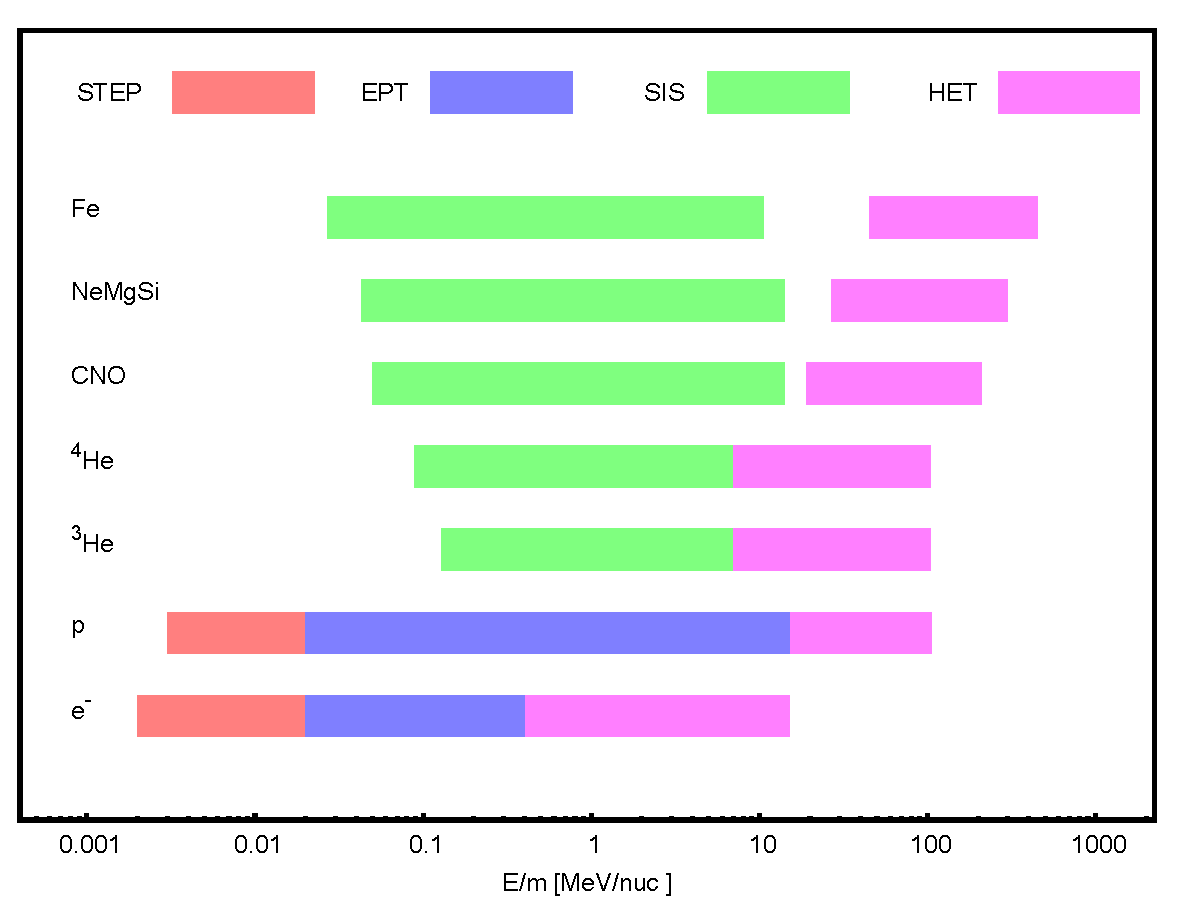
\includegraphics[width=0.7\textwidth]{images/epd-energy-ranges.pdf}
	\caption[\acs{EPD} energy coverage]{Energy coverage of the different sensors in the \ac{EPD} suite. Taken from \citet[Fig. 3]{RodriguezPacheco-2019-EPD}.}
	\label{fig:epd_energy_ranges}
\end{figure}

The double-ended \ac{HET} sensor head is shown in Figure \ref{fig:het-sensorhead}. Two of these sensors are installed onboard the \ac{SolO} spacecraft on the side decks, which provide four viewing directions: Sunward, antisunward, north and south. The sunward and antisunward fields of view are pointed \SI{35}{\degree} away from the radial direction, which corresponds to the mean direction of the nominal Parker spiral. The telescope consists of four silicon solid-state detectors (A1, B1, B2, A2) and a Bi$_4$Ge$_3$O$_{12}$ (BGO) scintillator (C) in the center. This setup is similar to \ac{MSL} (\autoref{sec:mslrad}), though there is no second plastic scintillator for the detection of neutral particles.



\begin{figure}
    \centering
    \subfloat[\acs{CAD} rendering of the \ac{HET} sensor head. Taken from \citet{RodriguezPacheco-2019-EPD}, Fig. 31.]{
    	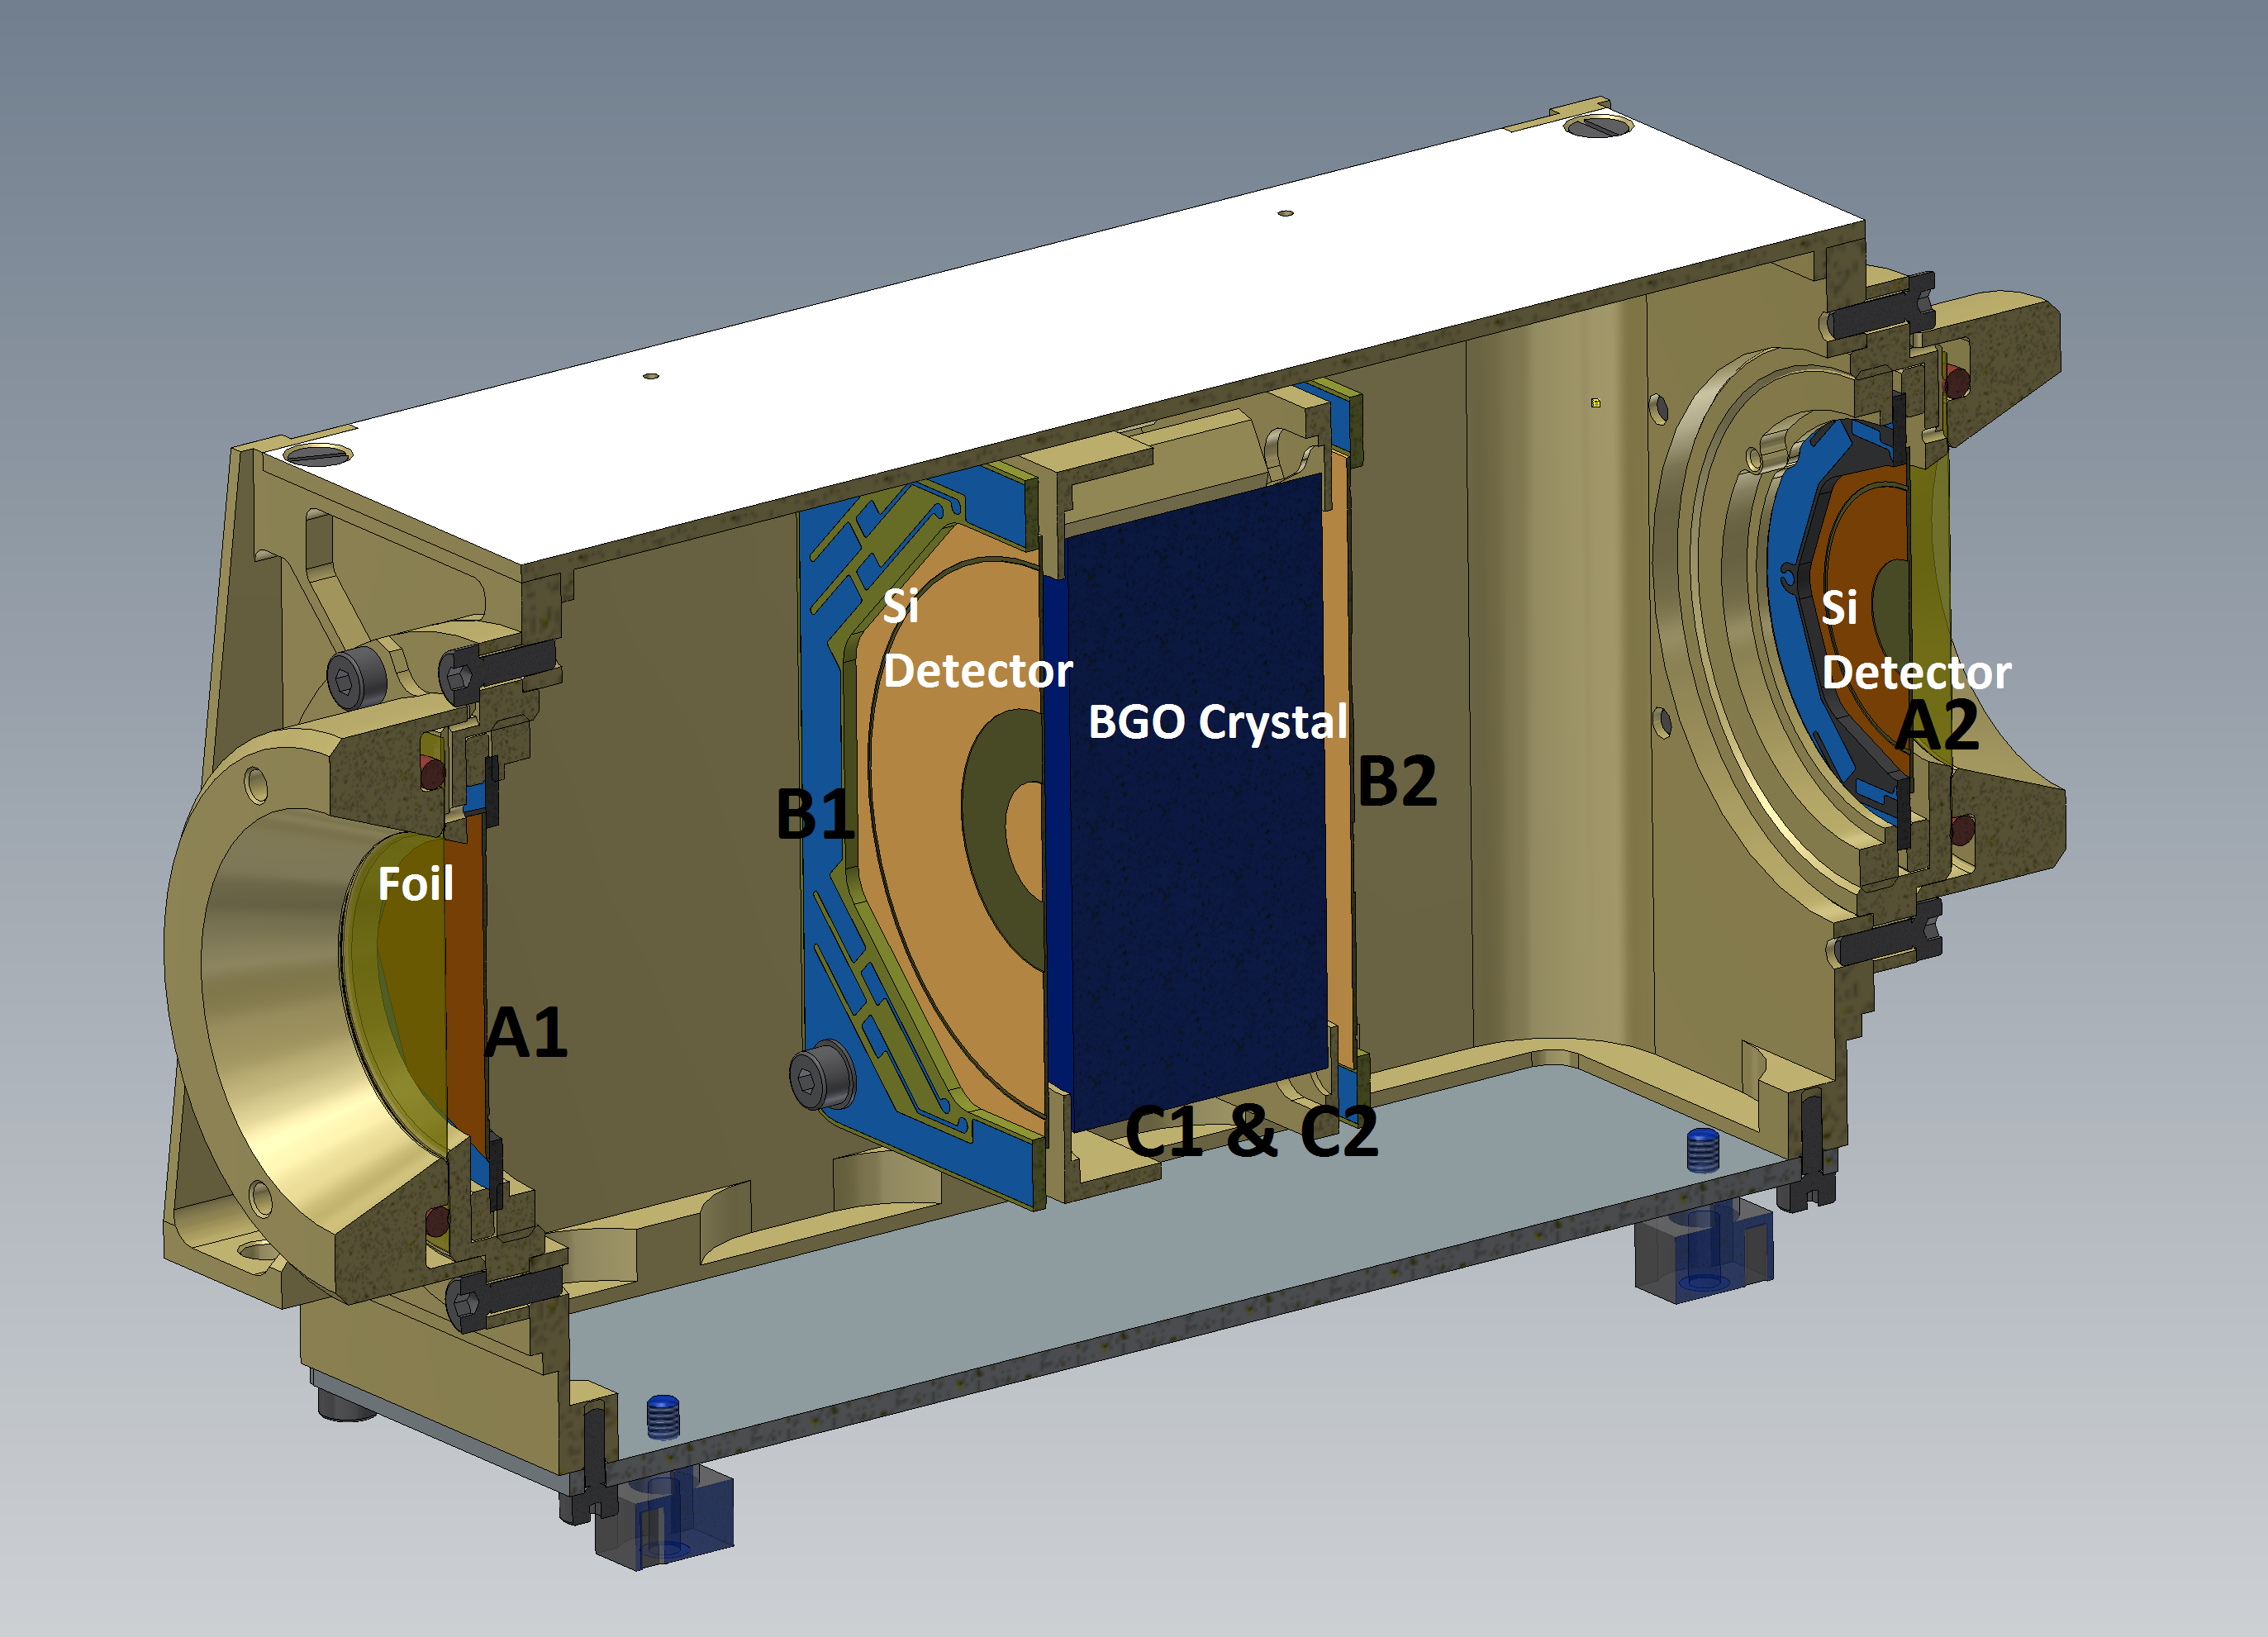
\includegraphics[width=0.6\textwidth]{images/het.png}
    	\label{subfig:het-sensorhead-cad}
    }\\
    \subfloat[Schematic diagram of the \ac{HET} sensor head]{
    	%\documentclass{standalone}
%\usepackage[dvipsnames]{xcolor}
%\usepackage{tikz}
%\usepackage{amsmath}
%\usepackage{siunitx}

%\usetikzlibrary{calc}
%\usetikzlibrary{decorations.pathmorphing}

%\definecolor{light-gray}{gray}{0.9}

%\begin{document}
\begin{tikzpicture}[scale=0.8]
    \tikzset{%
        add/.style args={#1 and #2}{
            to path={%
                ($(\tikztostart)!-#1!(\tikztotarget)$)--($(\tikztotarget)!-#2!(\tikztostart)$)%
                \tikztonodes},add/.default={.2 and .2}}
    }   
    
    \def\Sithickness{0.05}
    
    % A1
    \draw[fill=light-gray] (-\Sithickness, -0.87) rectangle (\Sithickness, 0.87) node[above,yshift=2mm]{A1};
    \draw (-\Sithickness, -0.4) -- (\Sithickness, -0.4);
    \draw (-\Sithickness, 0.4) -- (\Sithickness, 0.4);
    
    % B1
    \draw[fill=light-gray] (4.4-\Sithickness, -1.82) rectangle (4.4+\Sithickness, 1.82) node[above]{B1};
    \draw (4.4-\Sithickness, -0.4) -- (4.4+\Sithickness, -0.4);
    \draw (4.4-\Sithickness, 0.4) -- (4.4+\Sithickness, 0.4);
    \draw (4.4-\Sithickness, -0.87) -- (4.4+\Sithickness, -0.87);
    \draw (4.4-\Sithickness, 0.87) -- (4.4+\Sithickness, 0.87);
    
    % C
    \draw[fill=light-gray] (4.635, -1.75) rectangle ++(2, 3.5);
    \node[above, yshift=0.5mm] at (5.635, 1.75) {C};
    
    % B2
    \draw[fill=light-gray] (6.9-\Sithickness, -1.82) rectangle (6.9+\Sithickness, 1.82) node[above]{B2};
    \draw (6.9-\Sithickness, -0.4) -- (6.9+\Sithickness, -0.4);
    \draw (6.9-\Sithickness, 0.4) -- (6.9+\Sithickness, 0.4);
    \draw (6.9-\Sithickness, -0.87) -- (6.9+\Sithickness, -0.87);
    \draw (6.9-\Sithickness, 0.87) -- (6.9+\Sithickness, 0.87);
    
    % A2
    \draw[fill=light-gray] (11.3-\Sithickness, -0.87) rectangle (11.3+\Sithickness, 0.87) node[above,yshift=2mm]{A2};
    \draw (11.3-\Sithickness, -0.4) -- (11.3+\Sithickness, -0.4);
    \draw (11.3-\Sithickness, 0.4) -- (11.3+\Sithickness, 0.4);
    
    % FOV
    \draw[add=0.1 and 0, dashed, opacity=0.5] (0, -0.87) to (6.9, 1.82);
    \draw[add=0.1 and 0, dashed, opacity=0.5] (0, 0.87) to (6.9, -1.82);
    \draw[add=0.1 and 0, dashed, opacity=0.5] (11.3, -0.87) to (4.4, 1.82);
    \draw[add=0.1 and 0, dashed, opacity=0.5] (11.3, 0.87) to (4.4, -1.82);
    
    \draw[|<->|] (0, 0.87) ++ (180-21.45:0.5) arc (180-21.45:180+21.45:2.4+0.48) node[midway, left] {\small\SI{42.9}{\degree}};
    

    \draw[thick, red, -latex] (-0.2, 0.2) -- (4.4, 0.5);
    \draw[thick, green, -latex] (-0.2, 0) -- (5.7, 0.1);
    \draw[thick, blue, -latex] (-0.2, -0.2) -- (11.5, -0.5);
    \draw[thick, Aquamarine, -latex] (2.5, 2) -- (8.4, -2);
    \draw[thick, orange, -latex] (5.635, -2.3) -- (5.635, -1);
\end{tikzpicture}
%\end{document}
    	\label{subfig:het-sensorhead-diagram}
	}
    \caption[\acs{HET} sensor head]{\acs{HET} sensor head}
    \label{fig:het-sensorhead}
\end{figure}

Further details about the design of the \ac{HET} instrument can be found in \cite{Elftmann-2020-PhD}. 

\section{Neutron monitor measurements}
\label{sec:neutronmonitors}

\section{The STEREO Heliospheric Imagers}
\label{sec:stereohi}

\begin{figure}
    \centering
    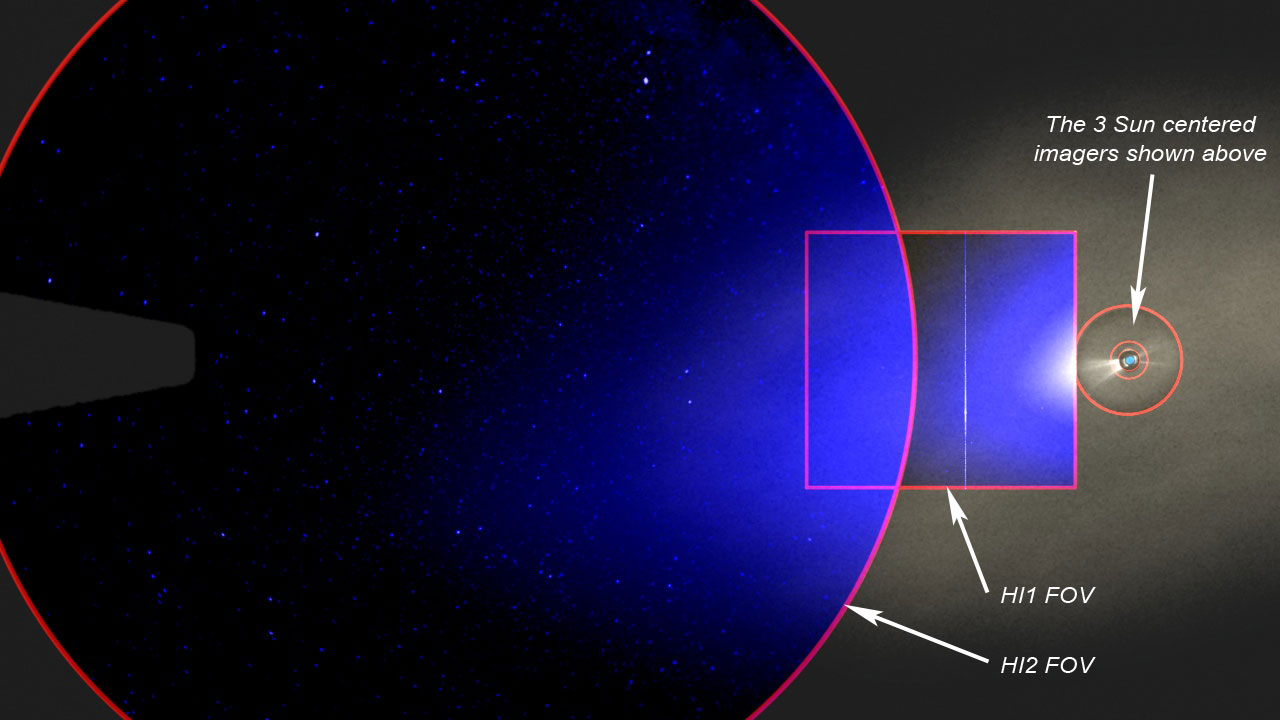
\includegraphics[width=0.8\linewidth]{images/secchi_fov}
    \caption[Fields of view of the \acs{STEREO} SECCHI telescopes]{Fields of view of the \ac{STEREO} SECCHI telescopes EUVI, COR1, COR2 (circles on the right side), and HI1 and HI2. Source: NASA/STEREO/GSFC}
    \label{fig:secchifov}
\end{figure}
